\section{Typo3}\label{Typo3}
Im Abschnitt \ref{PortalServerTypo3} wurde schon grundlegend auf Typo3 eingegangen. Es stellte sich im Abschnitt \ref{PortalserverAuswertung} heraus, dass Typo3 die besten M�glichkeiten bietet um ein modulares Supportsystem aufzubauen.

Im folgenden Kapitel wird genauer auf die Verwendung von Typo3 \ac{CMS} (im weiteren als Typo3 bezeichnet) eingegangen.
Hierbei wird auf die Roadmap von Typo3 eingegangen und gezeigt wie eine Typo3 Extension grundlegend entwickelt wird.

\subsection{Typo3 8.5}
Die momentan aktuelle \ac{LTS}-Version von Typo3 ist die Version 7, welche aktuell (Stand Dezember 2016) noch immer unterst�tzt wird.
Gleichzeitg wird eine neue \ac{LTS}-Version entwickelt, welche iterativ innerhalb der Version 8.x entsteht. Momentan ist die aktuelle Version 8.5, welche zum Beispiel einen neuen \ac{RTE}-Editor mitbringt. \cite{Typo85}

Im Verlauf des Jahres 2017, soll dann die neue \ac{LTS}-Version von Typo3 erscheinen. Da sich die Entwicklung des Supportportals vorraussichtlich bis Ende 2017 erstrecken wird, ist es nur logisch die Neuentwicklung auf den momentanen Zwischenversionen zu entwickeln, um bei der Fertigstellung m�glichst auf einer neuen \ac{LTS}-Version aufsetzen zu k�nnen.

\subsection{Extensions}
Es ist m�glich beinahe jede ben�tigte Funktion in Typo3 einzubauen. Dies geschieht �ber so genannte Extensions, welche den Funktionsumfang von Typo3 erweitern oder ver�ndern k�nnen.
Das Grundsystem, welches nach der Installation vorzufinden ist, basiert zum Teil schon auf Extensions, den sogenannten System-Extensions. Diese Extensions bringen grundlegende Funktionalit�ten in das Grundsystem ein und erweitern dieses. 

Das Auslagern von Funktionalit�ten in Extensions hat mehrere Vorteile. Zum einen entlastet es den System-Kern und macht diesen schlanker und �bersichtlicher. Zum anderen k�nnen Fehler in Extensions behoben werden, ohne das ganze System zu updaten. 

Konzepte von Typo3 Extensions sind zum einen die objektorienterte Programmierung und das \ac{MVC}-Prinzip.

\newpage
\paragraph{Objektorienterte Programmierung} sagt aus, dass alles und jedes im Programm auf Klassen basiert. Lediglich PHP-Funktionalit�ten wie finale Klassen oder die Sichtbarkeit "`private"' wird nicht unterst�tzt. 

Der gesammte PHP-Quellcode einer Extension ist Objektbasiert, nicht nur Modellklassen, sondern auch Konstroller oder Repositorys sind als Klassen abgebildet. 

\begin{wrapfigure}{r}{4cm}
\centering
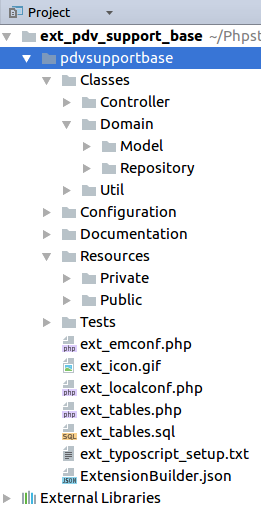
\includegraphics[width=4cm]{Bilder/projekt_struktur.png}
\caption{Extension Struktur}
\label{Extension Struktur}
\vspace{-40pt}
\end{wrapfigure}

\paragraph{Model-View-Controller} ist ein sehr bekanntes Strukturierungsmittel in der Informatik und kommt auch bei Typo3 Extensions zum Einsatz.
In einem Extension-Projekt, m�ssen alle Klassen innerhalb fester Pfade abgelegt werden.

In Abbildung \ref{Extension Struktur} ist die Struktur der Basis-Extension f�r das Supportportal zu sehen.

\subparagraph{Modellklassen,} welche nach dem \ac{MVC}-Prinzip reale Objekte verk�rpern, sind unter Classes/Domain/Model zu finden.
\subparagraph{Controller} sind unter Classes/Controller zu finden.
\subparagraph{Views,} welche bei Webseiten als HTML-Dateien realisiert werden, sind unter Resources/Private zu finden. Hier wiederum sind sie im Unterordner Templates zu finden. Eine Besonderheit bei Extensions ist, dass wiederkehrende Views so genannte "`Partials"' im Unterordner Partials zu finden sind. Partials werden innerhalb von Templates gerendert und dargsestellt.

Eine weitere Besonderheit sind die Repository-Klassen, welche unter /Classes/Domain/Repository zu finden sind. Sie stellen die Persistenzschicht zwischen Anwendung und Datenbank dar. Alle Lese- oder Schreiboperationen werden innerhalb der Repositorys durchgef�hrt. Typo3 stellt innerhalb der Repositorys viele dynamische Methode bereit, um Standardabfrage zu realisieren.

Um den Grundstock f�r eine neue eigene Extension zu legen, kann der Extension-Builder\footnote{\url{https://typo3.org/extensions/repository/view/extension_builder}} verwendet werden. Dieser baut unter Angabe des Domain-Modells und der Constroller die Grundextension auf, die dann mit Inhalt gef�llt werden kann.

\subsection{TypoScript}
\subsection{Fluid}\label{Fluid}
